\documentclass[12pt, a4paper]{article}
\usepackage[utf8]{inputenc}
\usepackage[spanish]{babel}
\usepackage{graphicx}

\begin{document}
\begin{titlepage}
\centering
{
\includegraphics[width=0.3\textwidth]{Imagenes/escudo_fi_color.png}\par}
\vspace{1cm}
{\bfseries\LARGE Universidad Nacional Autónoma de México\par}
\vspace{1cm}
{\scshape\Large Facultad de Ingeniería  \par}
\vspace{2cm}
{\scshape\Huge Proyecto 1: Ordenamiento Interno  \par}
\vspace{2cm}
\vfill
\raggedright
{\Large  Equipo 8: \par}
{\Large Integrantes: \par}
{\Large González Fernández, Jonathan Uriel \par}
{\Large Guillén Luna, Adair Isai \par}
{\Large Hernández Romero, Raúl \par}
\vfill
\raggedleft
{\Large Semestre 2022-2\par}
\end{titlepage}

\tableofcontents
\newpage
\section{Objetivo}\label{sec:objetivo}
Que el alumno implemente los algoritmos de ordenamiento externo y que conozca elementos para el manejo de archivos, aplique los conceptos generales de programación y desarrolle sus habilidades de trabajo en equipo.
\section{Introducción}\label{sec:intro}
\subsection{Ordenamiento}\label{subsec:ordenamiento}
El ordenamiento es la operación de reordenar los elementos en algún orden secuencial de acuerdo a un criterio de  ordenamiento. El propósito principal de un ordenamiento es el de facilitar las búsquedas de los miembros del conjunto ordenado.
\begin{figure}[h]
    \centering
    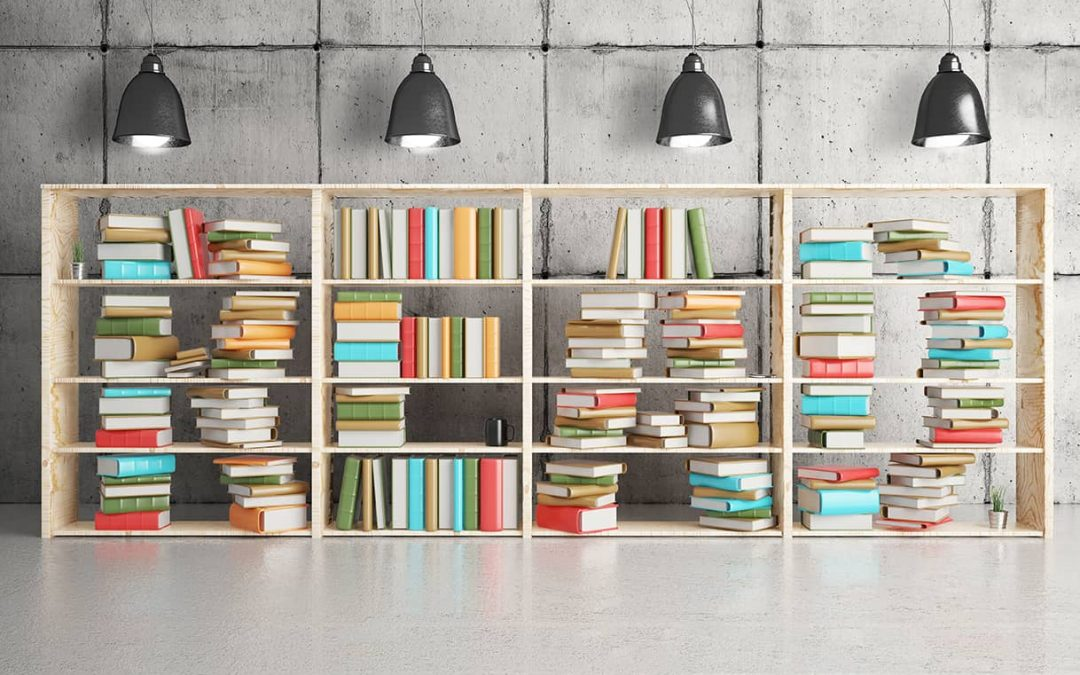
\includegraphics[width=0.3\textwidth]{Imagenes/ordenar.jpg}
    \caption{ordenar}
    \label{fig:img_orden}
\end{figure}
\subsection{Ordenamiento Interno}\label{sec:OrdenInterno}
El ordenamiento interno es aquel en donde  los valores a ordenar están en memoria secundaria (Unidades de almacenamiento, USB, cintas magnéticas, etc). El ordenamiento interno se hace cuando la cantidad de información a almacenar es muy grande para la memoria principal(RAM).
\begin{figure}[h]
    \centering
    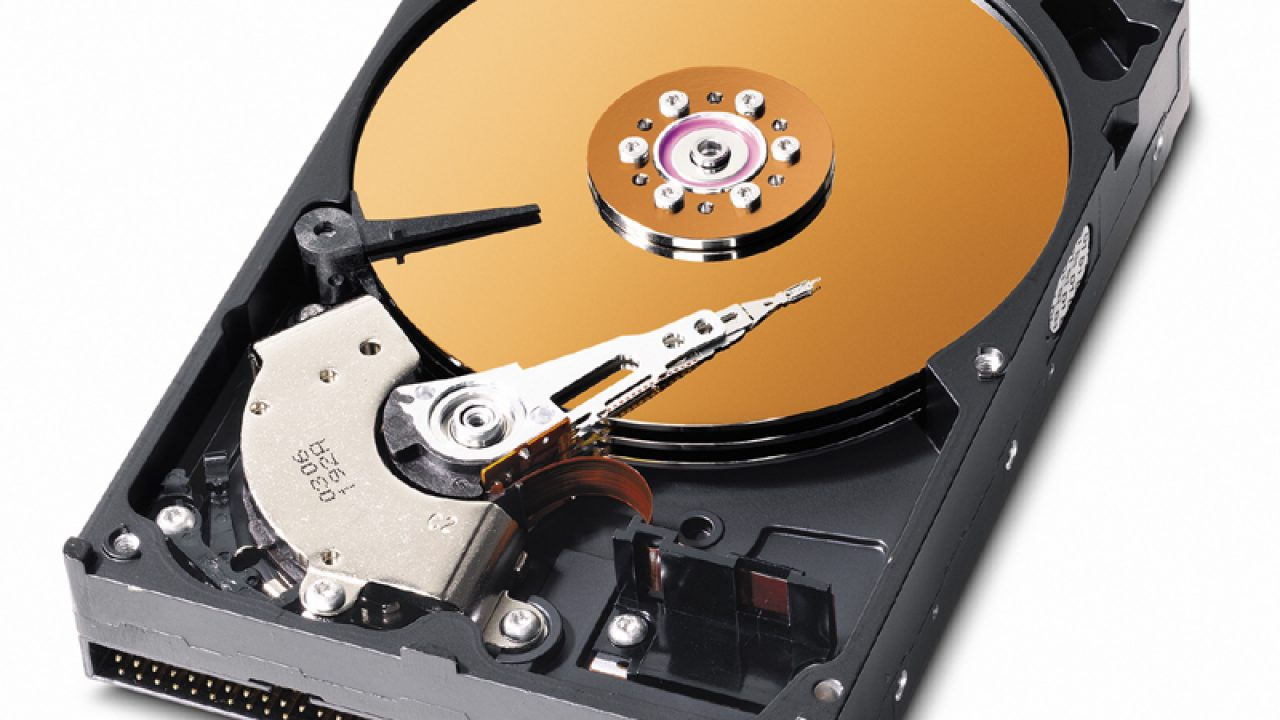
\includegraphics[width=0.3\textwidth]{Imagenes/disco_duro-1280x720.jpg}
    \caption{Disco Duro}
    \label{fig:discoDuro}
\end{figure}



\end{document}
